\documentclass[11pt,a4paper]{article}
\usepackage[utf8]{inputenc}
\usepackage[T1]{fontenc}
\usepackage[spanish]{babel}
\usepackage{geometry}
\geometry{left=1cm,right=1cm,top=1.2cm,bottom=0.8cm}
\usepackage{parskip}
\usepackage{hyperref}
\usepackage{enumitem}
\usepackage{graphicx}
\usepackage[most]{tcolorbox}
\usepackage{xcolor}
\usepackage{multicol}

% Definir colores pastel
\definecolor{pastelblue}{RGB}{173, 216, 230}
\definecolor{pastelgreen}{RGB}{152, 251, 152}
\definecolor{pastelpink}{RGB}{255, 182, 193}
\definecolor{pastelyellow}{RGB}{255, 255, 153}

% Comando personalizado para palabras en cajas
\newcommand{\roundedword}[2][pastelblue!30!white]{%
    \tcbox[enhanced, on line, colback=#1, colframe=black!70, 
           arc=3pt, boxrule=0.4pt, left=4pt, right=4pt,
           top=2pt, bottom=2pt]{#2}%
}



\hypersetup{
  colorlinks=true,
  linkcolor=blue,
  urlcolor=blue
}
\usepackage{sectsty}
\sectionfont{\large\bfseries}
\subsectionfont{\normalsize\bfseries}
\pagestyle{empty}
\pagenumbering{gobble}
\begin{document}

\begin{center}
  {\huge \textbf{Luis Huatay}}\\[6pt]
  \small
  Desarrollo de Software | Especialista GIS | Geomática\\
  \href{mailto:correo@ejemplo.com}{hsluis4326@gmail.com}
\end{center}

\noindent\makebox[\linewidth]{
  WhatsApp: (+51) 922 917 150
  \hfill
  \href{https://www.linkedin.com/in/lhuatay/}{LinkedIn}: linkedin.com/in/lhuatay \-  \href{https://github.com/1nfinit0}{GitHub}: github.com/1nfinit0}
\noindent\textcolor{black}{\rule{\linewidth}{0.1pt}}

Profesional en Sistemas de Información Geográfica (GIS) y actual pregrado en  Desarrollo de Software con experiencia en en desarrollo web (JavaScript, HTML/CSS), bases de datos (PostgreSQL, PostGIS) y automatización en Google Cloud y GitHub Actions. He publicado artículos científicos aplicando machine learning y datos satelitales, combinando investigación con buenas prácticas de ingeniería. Busco una posición como Ingeniero de Software para aportar en desarrollo backend, integración de datos y despliegue de aplicaciones.

\textbf{Algunas de mis habilidades:} 

\begin{center}
  \roundedword{JavaScript} \roundedword{Python} \roundedword{SQL} \roundedword{HTML5} \roundedword{CSS3} \roundedword{APIs REST} \roundedword{PostgreSQL} \roundedword{Data Science} \roundedword{Tailwind} \roundedword{Google Cloud Platform} \roundedword{Earth Engine API} \roundedword{Scraping} \roundedword{GitHub Actions} \roundedword{QGIS}
\end{center}
\vspace{-0.3cm}
\noindent\textcolor{black}{\rule{\linewidth}{0.1pt}}
\vspace{-0.9cm}
\section*{Experiencia laboral}
\begin{itemize}[left=15pt]
  \item \textbf{Desarrollador Web Independiente} \hfill \textbf{2021 -- actualidad}\\
    Desarrollo de soluciones web personalizadas incluyendo plataformas e-commerce, portafolios, geoportales y aplicaciones interactivas.
  \item \textbf{IEP JC - Docente de Matemática} \hfill \textbf{03/2022 -- actualidad}\\
    Fomento del pensamiento lógico y analítico en el nivel secundario como actividad paralela a mis labores profesionales y de investigación.
  \item \textbf{Centro Ecoturístico LOMAS DE PARAÍSO - Coordinador y Líder GIS} \hfill \textbf{01/2023 -- 11/2023}\\
    \textbf{Implementación de geoportal web} (HTML/CSS/JS + mapas interactivos) para gestión de información ecoturística. Lideré el equipo de producción de mapas temáticos y análisis espacial.
  \item \textbf{FISOTEC Solutions - Analista GIS} \hfill \textbf{03/2022 -- 07/2022}\\
    \textbf{Automatización de procesos geoespaciales} usando QGIS, Git y PostgreSQL/PostGIS. \textbf{Mejora de interoperabilidad} combinando flujos de trabajo en GitHub.
  \item \textbf{TECOM S.A.C. - Digitalización Cartográfica} \hfill \textbf{02/2021 -- 12/2021}\\
    Trabajo con ArcGIS y PostgreSQL en proyectos catastrales de más de 5 distritos de Lima.
\end{itemize}
\vspace{-0.5cm}
\section*{Educación}
\begin{itemize}[left=15pt]
  \item \textbf{Ingeniería de Software}, Universidad Tecnológica del Perú, Lima \hfill \textbf{Actualmente}
  \vspace{-0.3cm}
  \subitem Desarrollo Web, Bases de Datos, Gestión de Proyectos, Estadística, Estructuras de Datos y Algoritmos.
  \item \textbf{Técnico Profesional en Geomática}, Servicio Nacional para la Industria de la Construcción, \hfill \textbf{2022}
  \vspace{-0.3cm}
  \subitem Teledetección, Fotogrametría, Análisis Espacial, GIS, Cartografía Digital, Bases de Datos Geoespaciales.
\end{itemize}
\vspace{-0.2cm}
\section*{Proyectos e investigación}
\begin{itemize}[left=15pt]
  \item \textbf{Modeling Oceanic Anomalies and Vegetation Dynamics in Northern Peru} (2025) -- Artículo de revisión en MDPI - Climate sobre el modelamiento de anomalías oceánicas y dinámicas de vegetación en el norte de Perú. Paper en revisión. DOI: \href{https://www.mdpi.com/2673-7086/6/1/22}{Aquí}.
  \item \textbf{PE501088121-2024} (2025) -- Aplicación en Google Earth Engine para clasificación de cobertura agrícola; financiada por CONCYTEC-PROCIENCIA y respaldada por UTP, UNTRM y UPV. Link: \href{https://ee-hsluis4326.projects.earthengine.app/view/utpndvivstsm}{Aquí}.
  \item \textbf{Spatio-Temporal Changes in Agricultural Areas Under El Niño Events} (2025) -- Artículo publicado en Springer - CSOC 2025 sobre el ENSO y áreas agrícolas mediante estadística y teledetección. DOI: \href{https://doi.org/10.1007/978-3-032-04581-2_25}{Aquí}.
  \item \textbf{Líder del Semillero de Investigación en Ciencia de Datos Geo4All} (2025) -- Equipo de investigación enfocado a la capacitación en ciencia de datos, GIS y el desarrollo de proyectos de investigación.
  \item \textbf{Clasificación de Cobertura Agrícola} (2025) -- Proyecto que genera un modelo de clasificación supervisada de cobertura agrícola utilizando AlphaEarth y algoritmos de machine learning. Link: \href{https://github.com/1nfinit0/AlphaEarth-RandomForest-classifier---Lambayeque}{Aquí}.
\end{itemize}
% \begin{center}
%   Referencias disponibles a solicitud. Para ver mi trabajo puede acceder a mi \href{https://github.com/1nfinit0}{GitHub} o \href{https://www.linkedin.com/in/lhuatay/}{LinkedIn}.
% \end{center}
\newpage
\section*{Sobre mis proyectos}
\vspace{-0.5cm}
\noindent\textcolor{black}{\rule{\linewidth}{0.1pt}}
\begin{multicols}{2}

\begin{center}
  \textbf{Aplicación en Google Earth Engine para clasificación de cobertura agrícola}
\end{center}
\begin{center}
  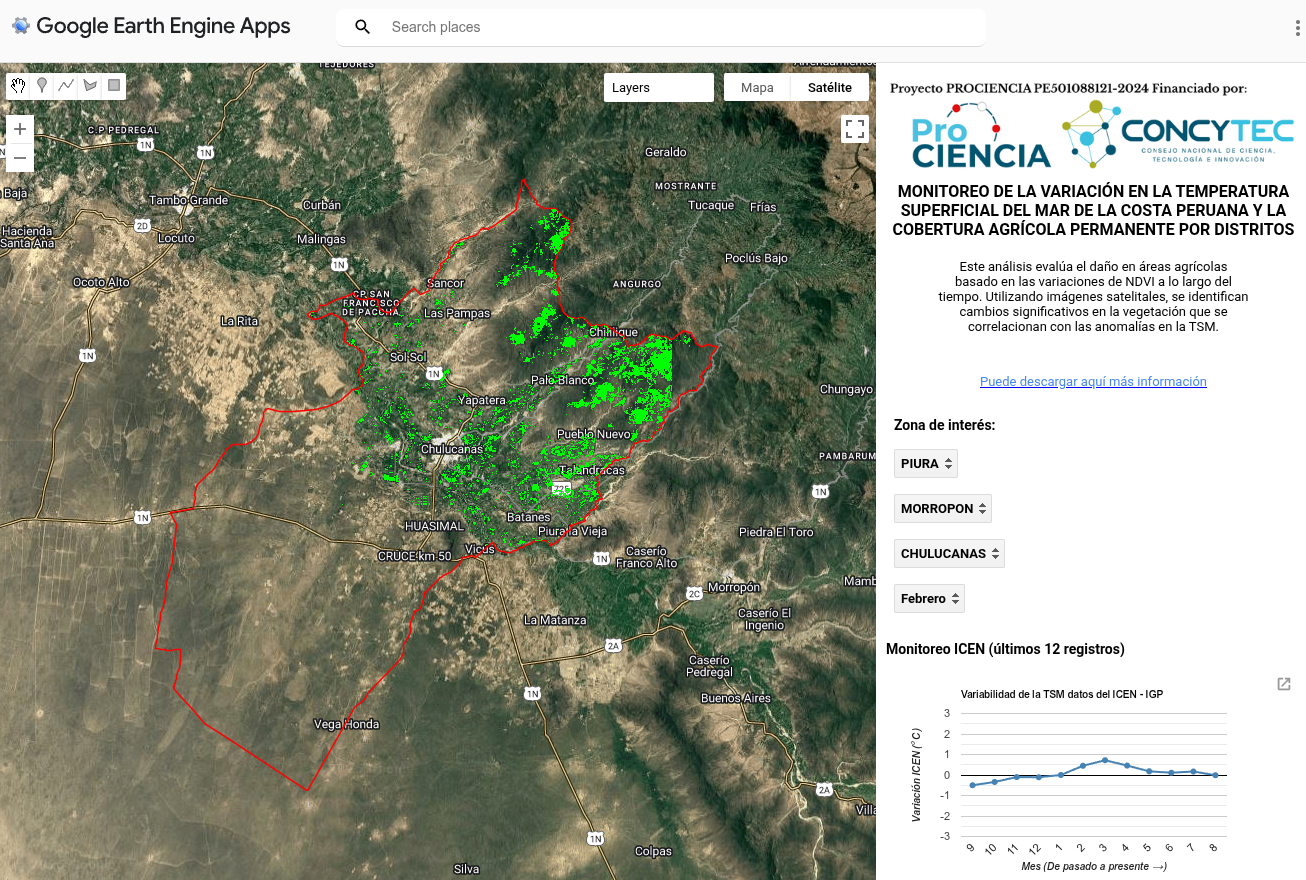
\includegraphics[width=\columnwidth]{assets/img1.png}
\end{center}
Como parte del proyecto PE501088121-2024 financiado por CONCYTEC-PROCIENCIA, desarrollé una aplicación bajo servicios de Google Cloud que permite la clasificación de cobertura agrícola en regiones específicas. La aplicación ofrece un producto basado en ciencia de datos que considera la persistencia del índice diferencial normalizado de vegetación capturado en una ventana temporal de 15 años que posteriormente se correlaciona con las anomalías de la temperatura superficial del mar.
\begin{center}
  \textit{Despliegue del aplicativo en el siguiente: \href{https://ee-hsluis4326.projects.earthengine.app/view/utpndvivstsm}{enlace}}
\end{center}
\noindent\textcolor{black}{\rule{\linewidth}{0.1pt}}
\begin{center}
  \textbf{Publicación de Artículo Científico en Springer | Software Engineering: Emerging Trends and Practices in System Development}
\end{center}
\begin{center}
  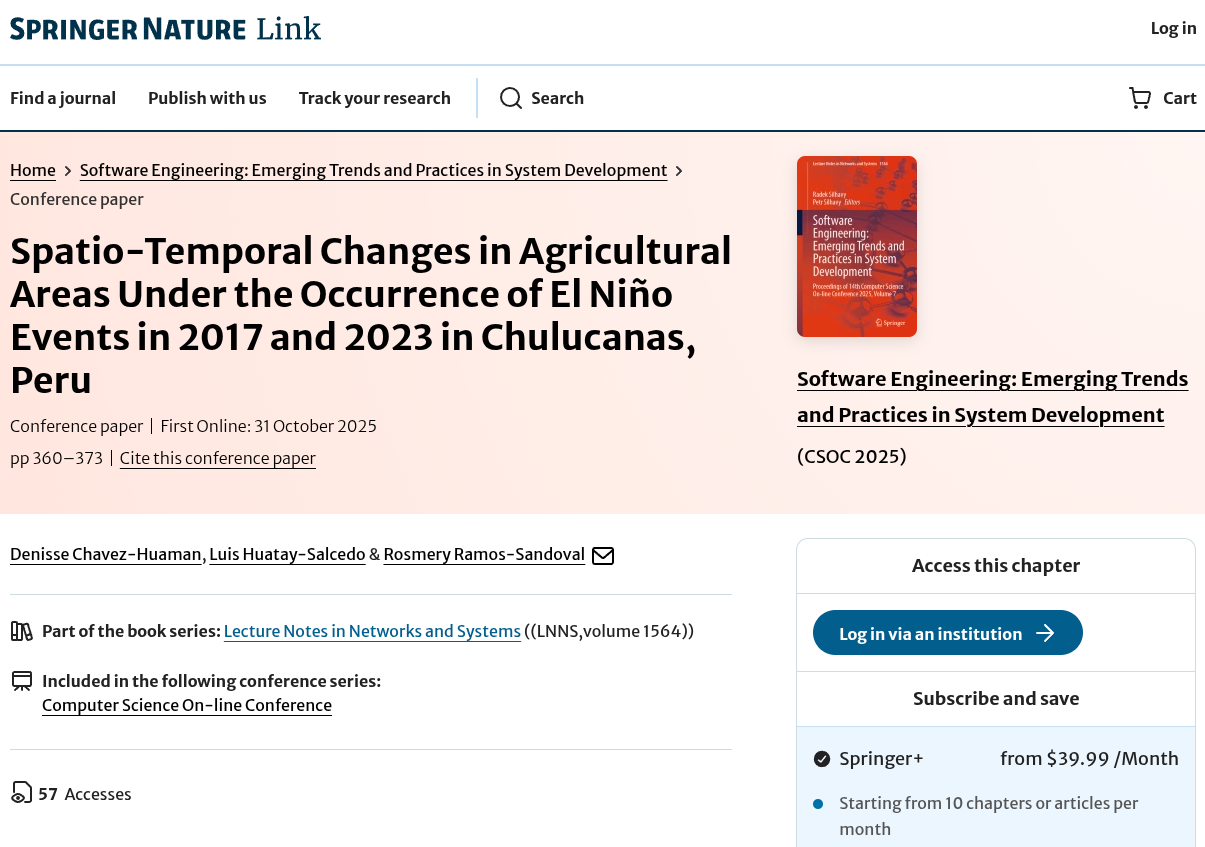
\includegraphics[width=\columnwidth]{assets/springer.png}
\end{center}
Estudio que aprovecha el modelo de clasificación generado anteriormente como motor de muestreo que servirá para la analisar el impacto del fenómeno El Niño Oscilación del Sur (ENSO) en la cobertura agrícola de la costa norte del Perú. El estudio demuestra el potencial del uso y aprovechamiento de estas técnicas que impactan directa y significativamente en los hogares agrícolas y comunidades afactadas por dicho fenómeno.
\begin{center}
  \textit{Puede acceder al artículo en el siguiente: \href{https://link.springer.com/chapter/10.1007/978-3-032-04581-2_25}{enlace}}
\end{center}
\columnbreak
\begin{center}
  \textbf{Modelo de clasificación supervisada utilizando técnicas de Machine Learning}
\end{center}
\begin{center}
  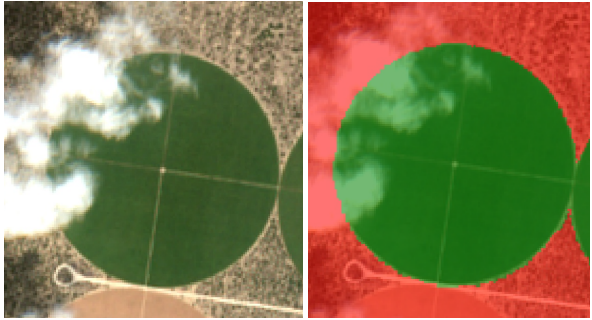
\includegraphics[width=\columnwidth]{assets/alpha.png}
\end{center}
Modelo de clasificación supervisada mediante RandomForest y entrenado con más de 300 etiquetas balanceadas, las muestras de entrenamiento toman datos del dataset AlphaEarth Foundations que integra en embeddings más de 60 características físicas y radiométricas del suelo. Dentro del proceso de evaluación del modelo se obtienen precisiones por encima del 99\% y matriz de confusión con taza de acierto de 10000 a 1.
\begin{center}
  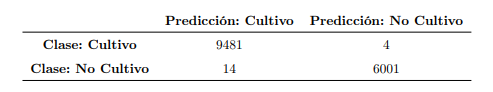
\includegraphics[width=0.8\columnwidth]{assets/confusion.png}
\end{center}
\begin{center}
  \textit{Puede acceder al repositorio en el siguiente: \href{https://github.com/1nfinit0/AlphaEarth-RandomForest-classifier---Lambayeque}{enlace}}
\end{center}
\noindent\textcolor{black}{\rule{\linewidth}{0.1pt}}
\begin{center}
  \textbf{Cartofy: Plataforma web como repositorio de mapas e información geoespacial}
\end{center}
\begin{center}
  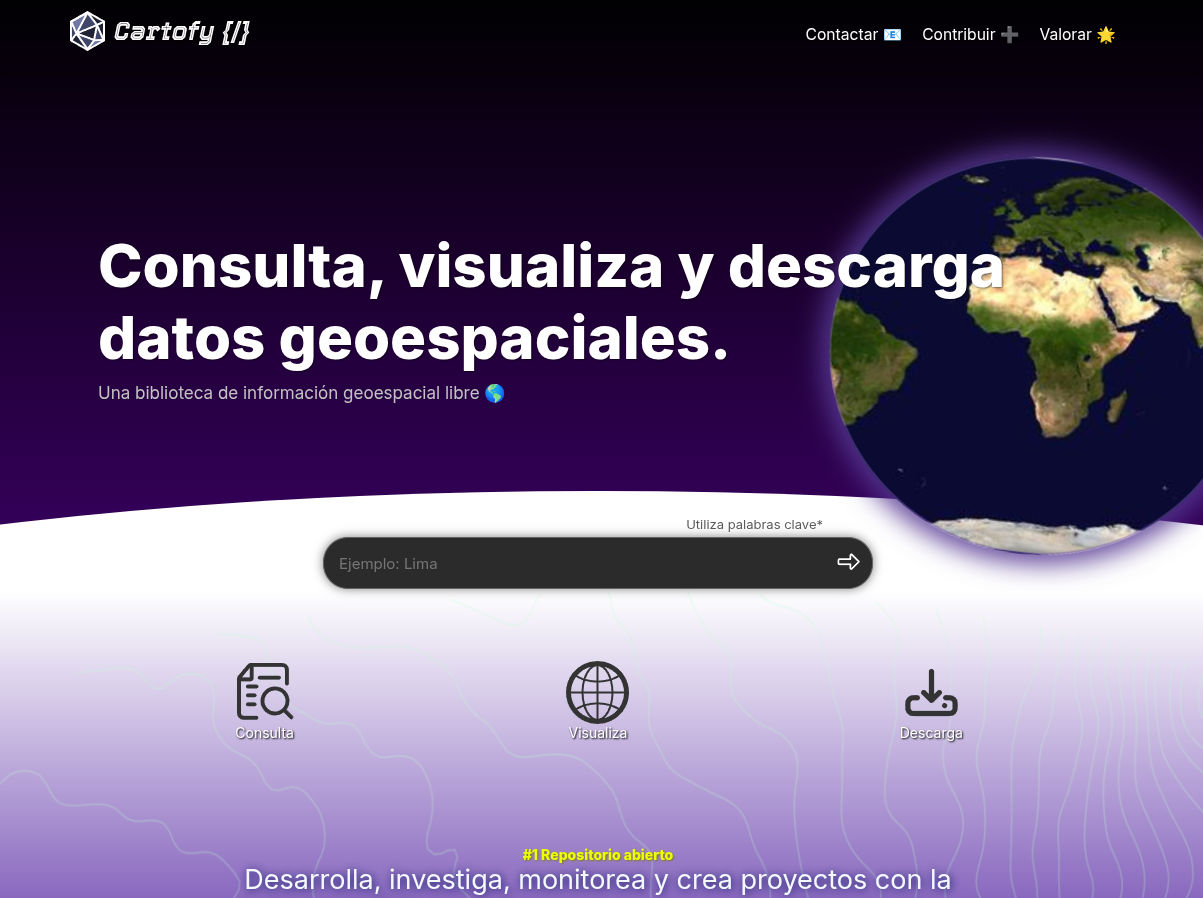
\includegraphics[width=\columnwidth]{assets/cartofy.png}
\end{center}
Desarrollé una plataforma web HTML/CSS y JS puro para la visualización y gestión de mapas temáticos interactivos. La plataforma permite a los usuarios explorar datos geoespaciales de manera intuitiva facilitando un espacio como repositorio de información geográfica de libre acceso, es una idea basada en BiblioCad.
\begin{center}
  \textit{Puede acceder al sitio web en el siguiente: \href{https://1nfinit0.github.io/cartofy/}{enlace}}
\end{center}
\end{multicols}
\newpage
\begin{multicols}{2}
\begin{center}
  \textbf{Portafolio personal de proyectos}
\end{center}
\begin{center}
  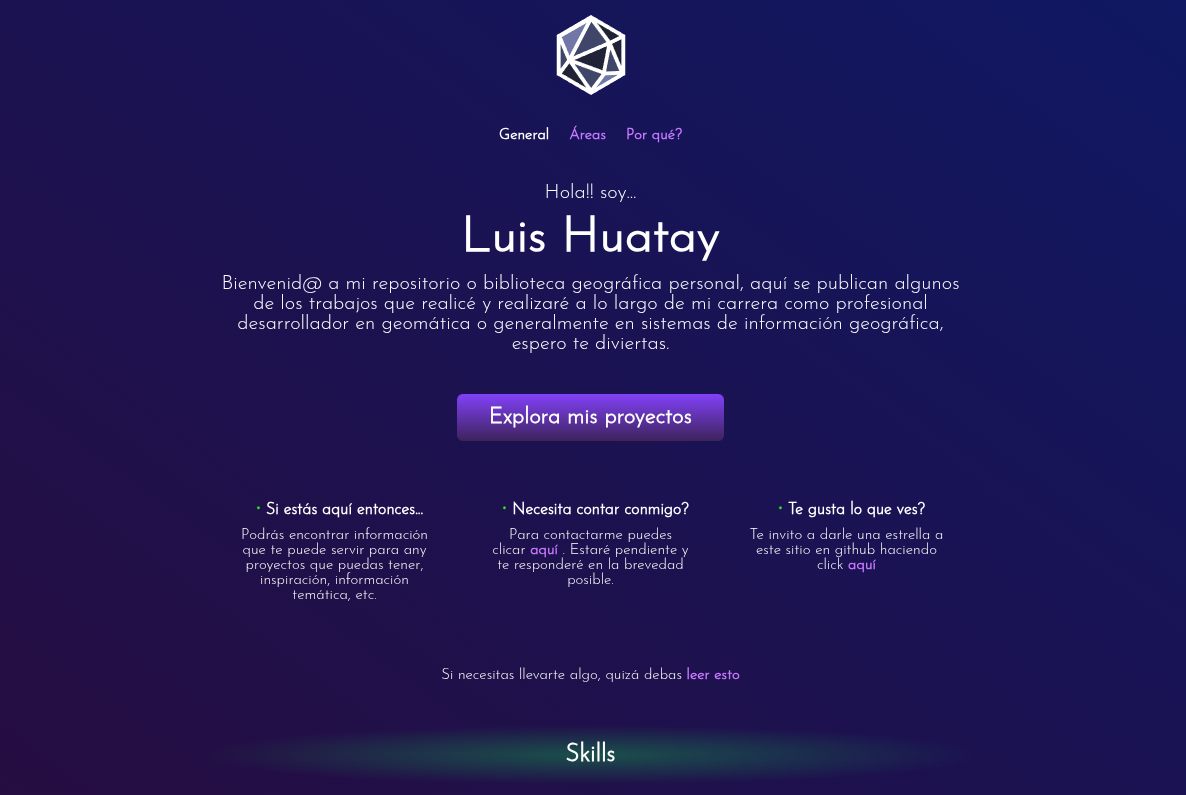
\includegraphics[width=\columnwidth]{assets/huatay.png}
\end{center}
Desarrollé mi portafolio de proyectos en en el cual muestro mi trabajo, este sitio fue uno de los primeros que hice durante mi formación en desarrollo web, está realizado con vanilla JavaScript y muestra una lista de servicios WMS tomados de entidades generadoras de información geográfica oficiales del Perú
\begin{center}
  \textit{Despliegue del sitio web en el siguiente: \href{https://1nfinit0.github.io/LuisH-mapCatalog/}{enlace}}
\end{center}
\vspace{-0.5cm}
\noindent\textcolor{black}{\rule{\linewidth}{0.1pt}}
\begin{center}
  \textbf{Metodología de consumo de modelos digitales de elevación (MDE) en web}
\end{center}
\begin{center}
  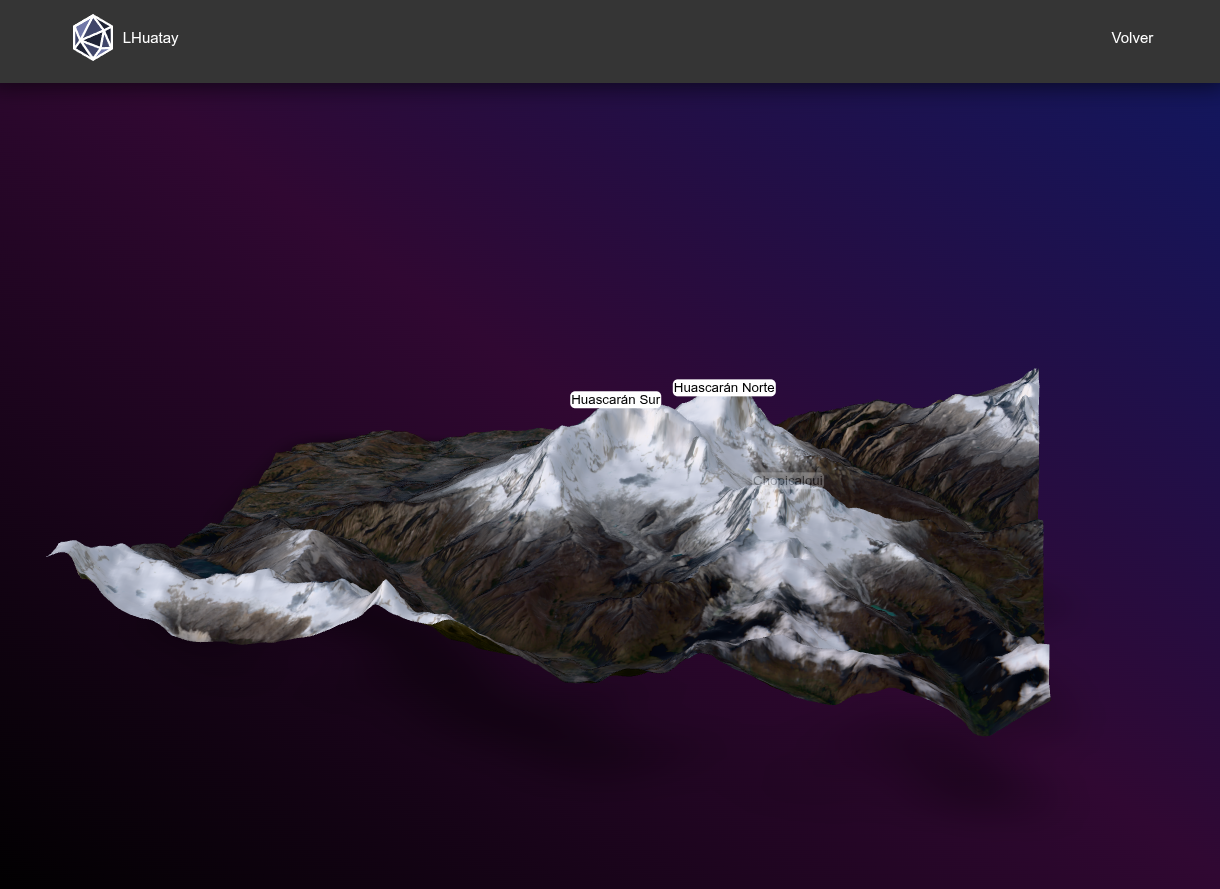
\includegraphics[width=\columnwidth]{assets/dem.png}
\end{center}
Dentro de mi catálogo de habilidades he desarrollado metodologías para el consumo de productos relacionados con el modelamiento 3D o fotogrametría en web, lo que me permite hacerlo con cualquier otro producto.
\begin{center}
  \textit{Puede acceder al artículo en el siguiente: \href{https://1nfinit0.github.io/peru_limites_departamentales/dirs/huascaran_3d/pantallaCompleta.html}{enlace}}
\end{center}
\noindent\textcolor{black}{\rule{\linewidth}{0.1pt}}
\begin{center}
  \textbf{Automatización de procesos de Scrapping en servicio alojados en Google Cloud}
\end{center}
\begin{center}
  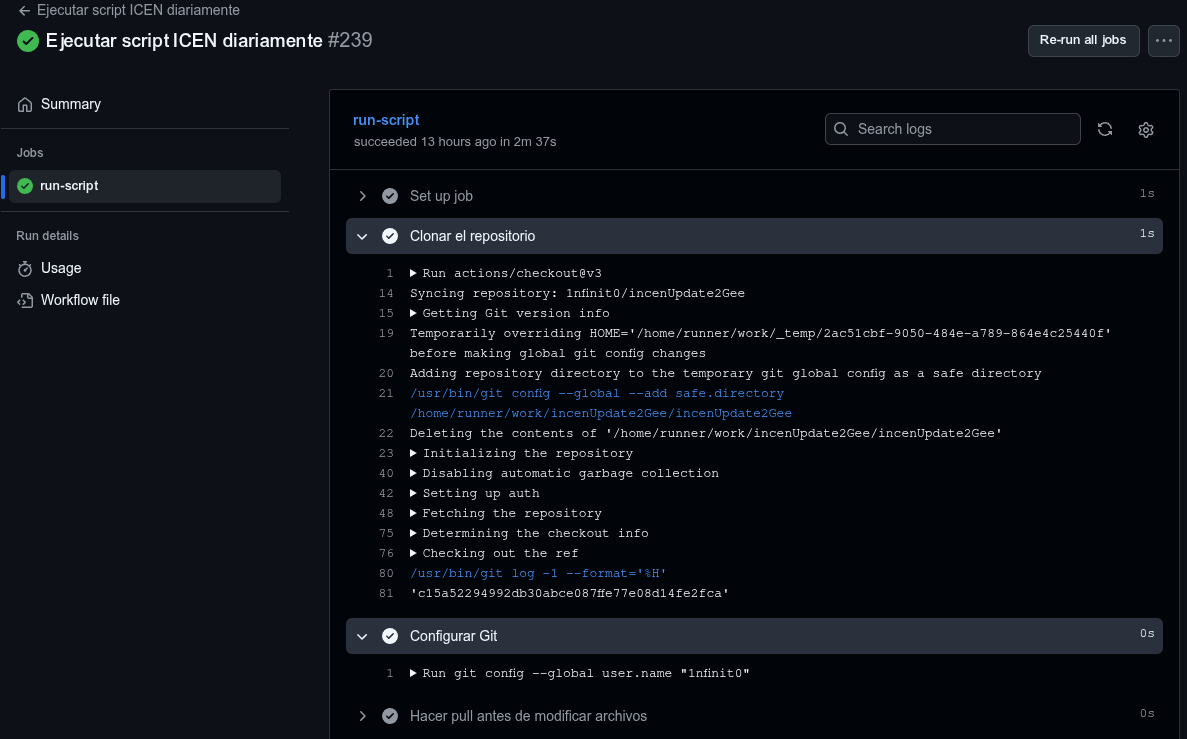
\includegraphics[width=\columnwidth]{assets/action.png}
\end{center}
Desarrollé técnicas avanzadas de interoperabilidad entre servicios externos a Google Cloud y automatización de estas. Estas técnicas reproducibles en en otros servicios similares muestra cómo aprovechar de una manera más precisa los servicios que ofrece la suit de Google.
\begin{center}
  \textit{Puede acceder al repositorio en el siguiente: \href{https://github.com/1nfinit0/incenUpdate2Gee/actions/runs/19954577960/job/57221093681}{enlace}}
\end{center}
\noindent\textcolor{black}{\rule{\linewidth}{0.1pt}}
\begin{center}
  \textbf{Geoportal: Lomas de Paraíso}
\end{center}
\begin{center}
  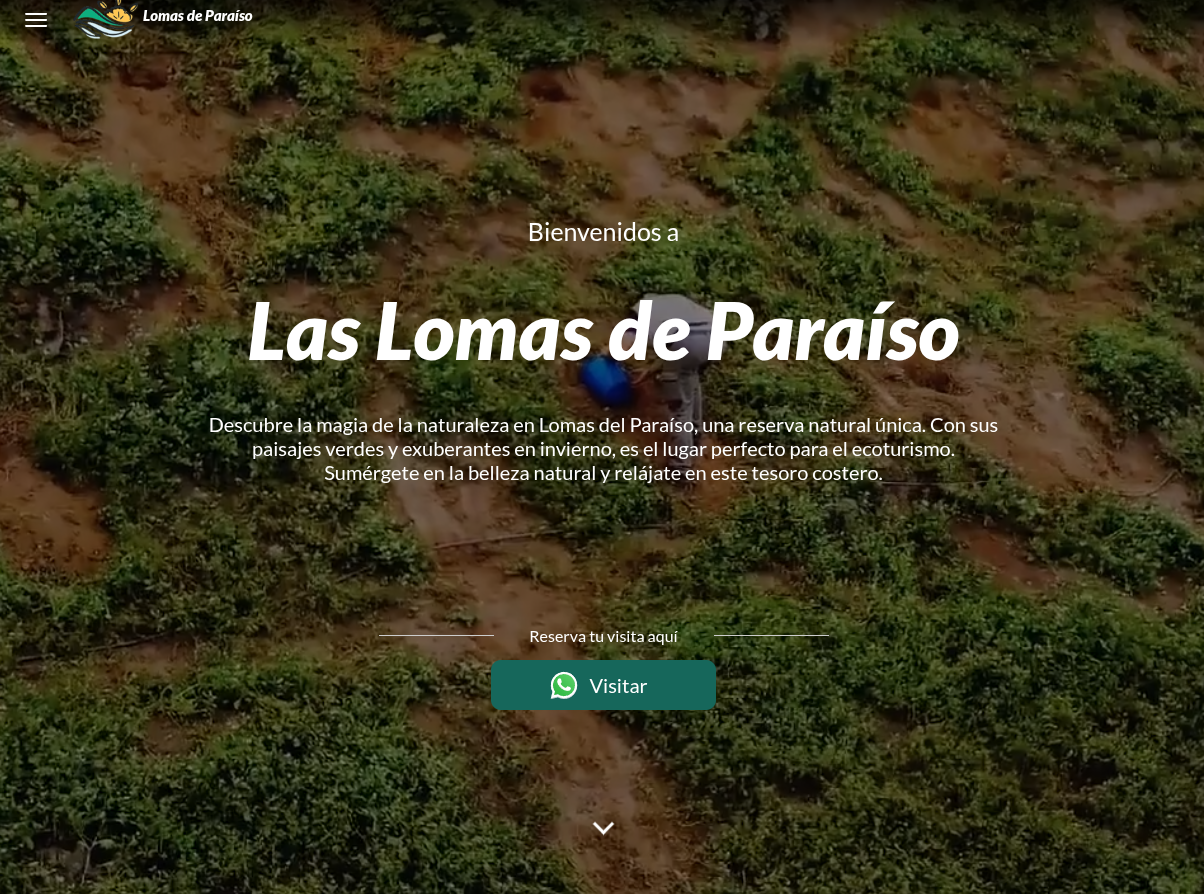
\includegraphics[width=0.9\columnwidth]{assets/web.png}
\end{center}
Desarrollé un geoportal para la visualización y gestión de información geoespacial de las Lomas de Paraíso. Este geoportal permite que las autoridades a cargado del circuito ecoturístico puedan registrar y visualizar la información que capturan en sus labores.
\begin{center}
  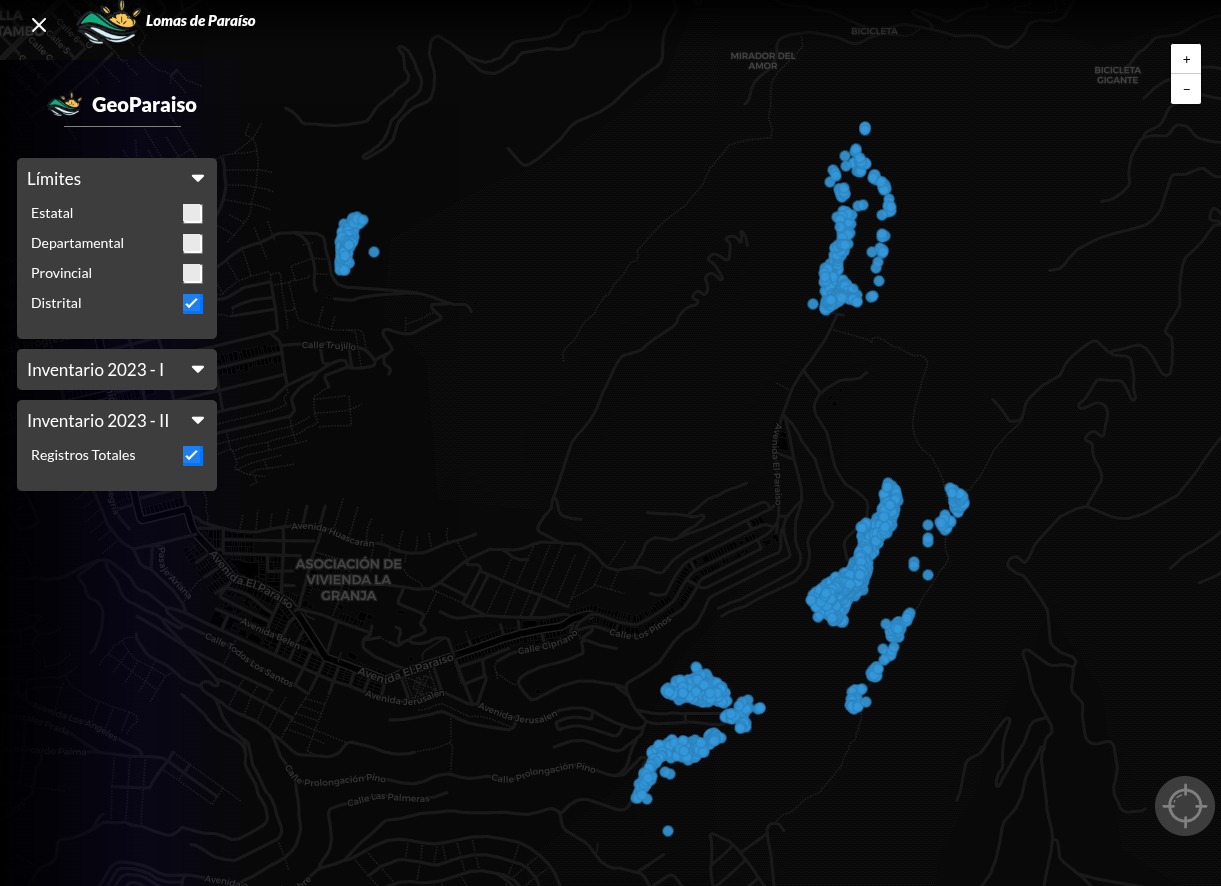
\includegraphics[width=0.9\columnwidth]{assets/portal.png}
\end{center}
\begin{center}
  \textit{Puede acceder al sitio web en el siguiente: \href{https://1nfinit0.github.io/LomasDeParaisoGeoPortal/}{enlace}}
\end{center}
\end{multicols}
\end{document}
